\iffalse
\documentclass{IEEEtran}

%\pagenumbering{roman}

\usepackage{xr}
\externaldocument{Classification}
\usepackage{cite}
\usepackage{amsmath}
\usepackage{tikz}
\usepackage{mathdots}
\usepackage{yhmath}
\usepackage{cancel}
\usepackage{color}
\usepackage{siunitx}
\usepackage{array}
\usepackage{multirow}
\usepackage{amssymb}
\usepackage{gensymb}
\usepackage{tabularx}
\usepackage{booktabs}
\usetikzlibrary{fadings}


\begin{document}
\fi
\section{Facial Expression Classification} \label{classification}
The classification portion of a facial expression recognition system at it's most basic level will take features as inputs and based on those inputs will make a determination of the expression displayed in the image. The input features will be the output of the feature extraction and selection stage and the determined class will be one of a pre-provided set of possibilities. In general, this type of classification has been performed either with a rule based scheme or using supervised machine learning classification algorithms. In the following section, rule-based and machine learning based classification methods will be examined.


\subsection{Rule Based Classification} \label{3-RBC}
\subsubsection{Probabilistic Model} As part of their system for robust facial expression recognition \cite{ioannou2007robust} implement a rule based classification model.
Instead of using the six archetypal expressions described by \cite{ekman1987universals} a quadrants of emotions wheel is used to classify emotions. A rule based probabilistic measure is used to determine which emotion is described in the image. The rules used by \cite{ioannou2007robust} consist of ranges corresponding to high, medium, and low activation of the facial animation parameters detected by the extraction phase. Because it is possible that not all possible defined features could be extracted from an image, \cite{ioannou2007robust} designed rules to ensure that only features that are known with a high degree of confidence have a significant impact on classification and those features that are not extracted or are extracted with lower degrees of confidence have less of an impact on the classification decision \cite{ioannou2007robust}. Based on the calculations of the rules outlined in \cite{ioannou2007robust}, the emotion is determined based on the $(x,y)$ point on the plot of activation emotion space as described in \cite{ioannou2007robust}. The $x$ and $y$ coordinates are determined based on the rules outlined in \cite{ioannou2007robust}.


\subsection{Machine Learning Based Classification} \label{3-LBC}
\subsubsection{Naive Bayesian Classifier}
A Naive Bayesian (NB) classification algorithm is used by \cite{lajevardi2012automatic} to classify images based on the output of each of the afore mentioned feature extraction methods. Naive Bayesian classifiers are Bayesian networks where all attributes are assumed to be independent \cite{zhang2004optimality}. Despite the fact that this assumption, called conditional independence, is rarely true in real world situations (there is typically some interdependence or correlation among features), Naive Bayesian classifiers have been shown to perform well compared to other classification methods \cite{zhang2004optimality}.

Bayesian classifiers make a classification determination based on the results of an evaluation function that examines the probability of each class given values fore each feature and selects the class with the highest probability. The algorithm stores the conditional probability, sometimes called the weight, of each feature given the class and for each iteration of training the conditional probabilities of each class are updated based on the result. It is an important characteristic of the Bayesian classifiers that the algorithm assumes that the features are statistically independent \cite{langley1992analysis}. Because of the fact that in most real world scenarios features are not statistically independent, initial work assumed that this classification method might produce poor results \cite{zhang2004optimality} \cite{langley1992analysis}. However, as shown in \cite{zhang2004optimality} that is not the case, rather Naive Bayesian classifiers have been shown to produce results on par with more sophisticated classification algorithms \cite{zhang2004optimality}.


The Naive Bayesian classifier is a probabilistic based model. First the probability of each class $c$ is calculated based on the given feature set $X = (x_1,x_2,...,x_n)$ as:

\begin{equation}
\label{eqn_nb_pclassGivenFeat}
p(c|X) = \frac{p(X|c)\:p(c)}{p(X)}
\end{equation}

\begin{center}
where
\end{center}
\begin{equation}
\label{eqn_nb_pclassGivenFeat}
p(c) = \frac{Number \: of \: Samples \: in \: Class \: c}{Total \: Number \: of \: Samples}
\end{equation}

 \cite{lajevardi2012automatic} and $p(X)$ is equal for all classes and can therefore be ignored \cite{rish2001empirical}.


The evaluation function $p(X|c)$ accounts for the probability of each feature set $X$ given each class $c$. This is often called the conditional probability. The function for the conditional probability is given as:

\begin{equation}
\label{eqn_nb_cprob}
p(X|c) = \prod_{i=1}^n p(x_i|c)
\end{equation}

and the class $C$ is determined by the maximum value of $p(c|X)$ after evaluating all classes $c$ where the total number of classes $k$ is shown as:

\begin{equation}
\label{eqn_nb_classify}
C = max \{p(c_1|X),...,p(c_k|X)\}
\end{equation}

\subsubsection{Neural Network Classifier}
Neural networks are a popular machine learning algorithm used for multi-class classification problem. Neural networks have been used been used in Face Detection, Feature Extraction and Classification stages of other facial expression recognition systems with success. \cite{rowley1998nn} used neural networks for face detection, \cite{xie2019deep}, \cite{ioannou2007robust}, and \cite{yu2018eye} used neural networks for feature extraction and \cite{alazzawi2018performance} and \cite{parkhi2015deep} used neural networks for face recognition. 

Neural networks, modeled after the function of neurons in the human brain, are networks of connected nodes called perceptrons \cite{pal1992multilayer}. There is an input layer of nodes where each node corresponds to one feature of input, followed by one or more ``hidden'' layers of nodes that connect prior layers to the next with weighted connections, the final layer is the output layer which encodes the classification \cite{pal1992multilayer}.


\begin{figure}
\centering


\tikzset{every picture/.style={line width=0.75pt}} %set default line width to 0.75pt        

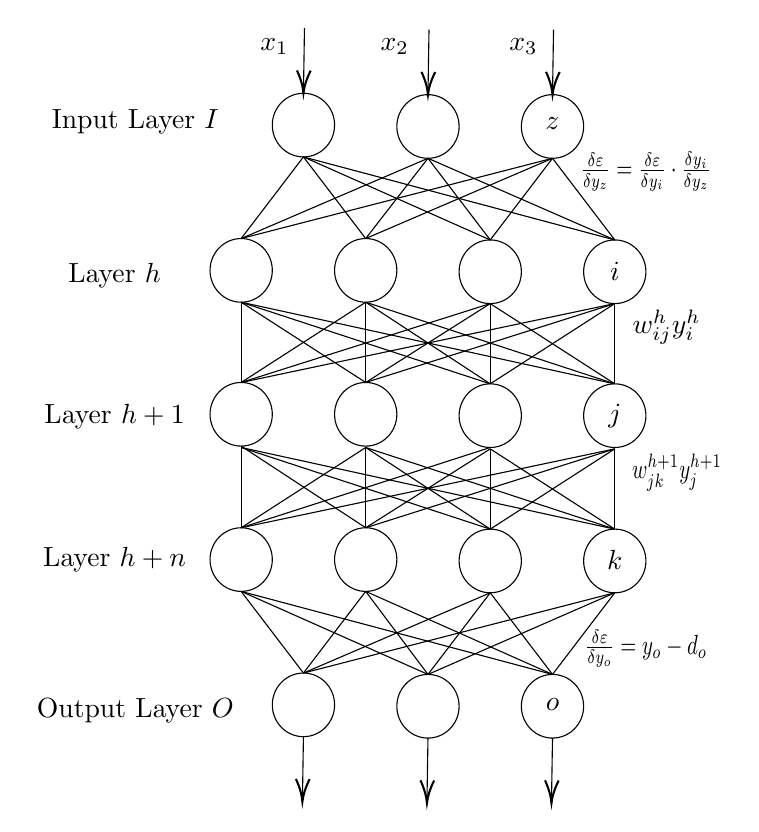
\begin{tikzpicture}[x=0.75pt,y=0.75pt,yscale=-1,xscale=1]
%uncomment if require: \path (0,918.3333435058594); %set diagram left start at 0, and has height of 918.3333435058594

%Flowchart: Connector [id:dp1999782616308523] 
\draw   (140,72.67) .. controls (140,64.2) and (146.72,57.33) .. (155,57.33) .. controls (163.28,57.33) and (170,64.2) .. (170,72.67) .. controls (170,81.14) and (163.28,88) .. (155,88) .. controls (146.72,88) and (140,81.14) .. (140,72.67) -- cycle ;
%Flowchart: Connector [id:dp4638526881382943] 
\draw   (200,73.33) .. controls (200,64.86) and (206.72,58) .. (215,58) .. controls (223.28,58) and (230,64.86) .. (230,73.33) .. controls (230,81.8) and (223.28,88.67) .. (215,88.67) .. controls (206.72,88.67) and (200,81.8) .. (200,73.33) -- cycle ;
%Flowchart: Connector [id:dp34953252838292914] 
\draw   (260,73.33) .. controls (260,64.86) and (266.72,58) .. (275,58) .. controls (283.28,58) and (290,64.86) .. (290,73.33) .. controls (290,81.8) and (283.28,88.67) .. (275,88.67) .. controls (266.72,88.67) and (260,81.8) .. (260,73.33) -- cycle ;
%Flowchart: Connector [id:dp8088598815308989] 
\draw   (110,142.67) .. controls (110,134.2) and (116.72,127.33) .. (125,127.33) .. controls (133.28,127.33) and (140,134.2) .. (140,142.67) .. controls (140,151.14) and (133.28,158) .. (125,158) .. controls (116.72,158) and (110,151.14) .. (110,142.67) -- cycle ;
%Flowchart: Connector [id:dp8319087784289663] 
\draw   (170,142.67) .. controls (170,134.2) and (176.72,127.33) .. (185,127.33) .. controls (193.28,127.33) and (200,134.2) .. (200,142.67) .. controls (200,151.14) and (193.28,158) .. (185,158) .. controls (176.72,158) and (170,151.14) .. (170,142.67) -- cycle ;
%Flowchart: Connector [id:dp08077051351305586] 
\draw   (230,143.33) .. controls (230,134.86) and (236.72,128) .. (245,128) .. controls (253.28,128) and (260,134.86) .. (260,143.33) .. controls (260,151.8) and (253.28,158.67) .. (245,158.67) .. controls (236.72,158.67) and (230,151.8) .. (230,143.33) -- cycle ;
%Flowchart: Connector [id:dp39097424978035744] 
\draw   (290,143.33) .. controls (290,134.86) and (296.72,128) .. (305,128) .. controls (313.28,128) and (320,134.86) .. (320,143.33) .. controls (320,151.8) and (313.28,158.67) .. (305,158.67) .. controls (296.72,158.67) and (290,151.8) .. (290,143.33) -- cycle ;
%Flowchart: Connector [id:dp16069978515034533] 
\draw   (110,212) .. controls (110,203.53) and (116.72,196.67) .. (125,196.67) .. controls (133.28,196.67) and (140,203.53) .. (140,212) .. controls (140,220.47) and (133.28,227.33) .. (125,227.33) .. controls (116.72,227.33) and (110,220.47) .. (110,212) -- cycle ;
%Flowchart: Connector [id:dp9151618610910661] 
\draw   (170,212) .. controls (170,203.53) and (176.72,196.67) .. (185,196.67) .. controls (193.28,196.67) and (200,203.53) .. (200,212) .. controls (200,220.47) and (193.28,227.33) .. (185,227.33) .. controls (176.72,227.33) and (170,220.47) .. (170,212) -- cycle ;
%Flowchart: Connector [id:dp3662992262656779] 
\draw   (230,212.67) .. controls (230,204.2) and (236.72,197.33) .. (245,197.33) .. controls (253.28,197.33) and (260,204.2) .. (260,212.67) .. controls (260,221.14) and (253.28,228) .. (245,228) .. controls (236.72,228) and (230,221.14) .. (230,212.67) -- cycle ;
%Flowchart: Connector [id:dp9663626257935529] 
\draw   (290,212.67) .. controls (290,204.2) and (296.72,197.33) .. (305,197.33) .. controls (313.28,197.33) and (320,204.2) .. (320,212.67) .. controls (320,221.14) and (313.28,228) .. (305,228) .. controls (296.72,228) and (290,221.14) .. (290,212.67) -- cycle ;
%Flowchart: Connector [id:dp43857777178268953] 
\draw   (110,282) .. controls (110,273.53) and (116.72,266.67) .. (125,266.67) .. controls (133.28,266.67) and (140,273.53) .. (140,282) .. controls (140,290.47) and (133.28,297.33) .. (125,297.33) .. controls (116.72,297.33) and (110,290.47) .. (110,282) -- cycle ;
%Flowchart: Connector [id:dp650814973856433] 
\draw   (170,282) .. controls (170,273.53) and (176.72,266.67) .. (185,266.67) .. controls (193.28,266.67) and (200,273.53) .. (200,282) .. controls (200,290.47) and (193.28,297.33) .. (185,297.33) .. controls (176.72,297.33) and (170,290.47) .. (170,282) -- cycle ;
%Flowchart: Connector [id:dp5987637413592404] 
\draw   (230,282.67) .. controls (230,274.2) and (236.72,267.33) .. (245,267.33) .. controls (253.28,267.33) and (260,274.2) .. (260,282.67) .. controls (260,291.14) and (253.28,298) .. (245,298) .. controls (236.72,298) and (230,291.14) .. (230,282.67) -- cycle ;
%Flowchart: Connector [id:dp7896686745607286] 
\draw   (290,282.67) .. controls (290,274.2) and (296.72,267.33) .. (305,267.33) .. controls (313.28,267.33) and (320,274.2) .. (320,282.67) .. controls (320,291.14) and (313.28,298) .. (305,298) .. controls (296.72,298) and (290,291.14) .. (290,282.67) -- cycle ;
%Flowchart: Connector [id:dp1684405299484435] 
\draw   (140,352) .. controls (140,343.53) and (146.72,336.67) .. (155,336.67) .. controls (163.28,336.67) and (170,343.53) .. (170,352) .. controls (170,360.47) and (163.28,367.33) .. (155,367.33) .. controls (146.72,367.33) and (140,360.47) .. (140,352) -- cycle ;
%Flowchart: Connector [id:dp4455266057616105] 
\draw   (200,352.67) .. controls (200,344.2) and (206.72,337.33) .. (215,337.33) .. controls (223.28,337.33) and (230,344.2) .. (230,352.67) .. controls (230,361.14) and (223.28,368) .. (215,368) .. controls (206.72,368) and (200,361.14) .. (200,352.67) -- cycle ;
%Flowchart: Connector [id:dp7841543637598003] 
\draw   (260,352.67) .. controls (260,344.2) and (266.72,337.33) .. (275,337.33) .. controls (283.28,337.33) and (290,344.2) .. (290,352.67) .. controls (290,361.14) and (283.28,368) .. (275,368) .. controls (266.72,368) and (260,361.14) .. (260,352.67) -- cycle ;
%Straight Lines [id:da7296614712186866] 
\draw    (155,88) -- (305,128) ;


%Straight Lines [id:da95549702416122] 
\draw    (155,88) -- (245,128) ;


%Straight Lines [id:da31187192688984444] 
\draw    (155,88) -- (185,127.33) ;


%Straight Lines [id:da0015227165925528752] 
\draw    (155,88) -- (125,127.33) ;


%Straight Lines [id:da795209449448232] 
\draw    (215,88.67) -- (305,128) ;


%Straight Lines [id:da640811476633236] 
\draw    (215,88.67) -- (245,128) ;


%Straight Lines [id:da10656368843132613] 
\draw    (185,127.33) -- (215,88.67) ;


%Straight Lines [id:da9817044619174213] 
\draw    (125,127.33) -- (215,88.67) ;


%Straight Lines [id:da16802623039360554] 
\draw    (275,88.67) -- (305,128) ;


%Straight Lines [id:da2864597359556491] 
\draw    (245,128) -- (275,88.67) ;


%Straight Lines [id:da34330068305222183] 
\draw    (185,127.33) -- (275,88.67) ;


%Straight Lines [id:da1424082061266967] 
\draw    (125,127.33) -- (275,88.67) ;


%Straight Lines [id:da9074039317146441] 
\draw    (125,158) -- (305,197.33) ;


%Straight Lines [id:da11181766109306235] 
\draw    (125,158) -- (245,197.33) ;


%Straight Lines [id:da09207421728387355] 
\draw    (125,158) -- (185,196.67) ;


%Straight Lines [id:da9269227384207284] 
\draw    (125,158) -- (125,196.67) ;


%Straight Lines [id:da6311242197193294] 
\draw    (185,158) -- (305,197.33) ;


%Straight Lines [id:da7157468882618694] 
\draw    (185,158) -- (245,197.33) ;


%Straight Lines [id:da8211510400805617] 
\draw    (185,158) -- (185,196.67) ;


%Straight Lines [id:da4109257013165539] 
\draw    (125,196.67) -- (185,158) ;


%Straight Lines [id:da7823810278397867] 
\draw    (245,158.67) -- (305,197.33) ;


%Straight Lines [id:da46603858418459443] 
\draw    (245,158.67) -- (245,197.33) ;


%Straight Lines [id:da4577071036682243] 
\draw    (185,196.67) -- (245,158.67) ;


%Straight Lines [id:da18689530464740267] 
\draw    (125,196.67) -- (245,158.67) ;


%Straight Lines [id:da33821056740652056] 
\draw    (305,158.67) -- (305,197.33) ;


%Straight Lines [id:da2773851803950296] 
\draw    (245,197.33) -- (305,158.67) ;


%Straight Lines [id:da7150342703655499] 
\draw    (185,196.67) -- (305,158.67) ;


%Straight Lines [id:da8985268693084112] 
\draw    (125,196.67) -- (305,158.67) ;


%Straight Lines [id:da7202780883807927] 
\draw    (125,228) -- (305,267.33) ;


%Straight Lines [id:da6556929946494692] 
\draw    (125,228) -- (245,267.33) ;


%Straight Lines [id:da8424315192219356] 
\draw    (125,227.33) -- (185,266.67) ;


%Straight Lines [id:da030649836950903175] 
\draw    (125,227.33) -- (125,266.67) ;


%Straight Lines [id:da10601673057451544] 
\draw    (185,228) -- (305,267.33) ;


%Straight Lines [id:da02545107643660449] 
\draw    (185,228) -- (245,267.33) ;


%Straight Lines [id:da29662255491602596] 
\draw    (185,228) -- (185,266.67) ;


%Straight Lines [id:da95922252204627] 
\draw    (125,266.67) -- (185,228) ;


%Straight Lines [id:da1410434965434737] 
\draw    (245,228.67) -- (305,267.33) ;


%Straight Lines [id:da8521452004546188] 
\draw    (245,228.67) -- (245,267.33) ;


%Straight Lines [id:da19151816481183603] 
\draw    (185,266.67) -- (245,228.67) ;


%Straight Lines [id:da5052208204128217] 
\draw    (125,266.67) -- (245,228) ;


%Straight Lines [id:da6133383723546693] 
\draw    (305,228.67) -- (305,267.33) ;


%Straight Lines [id:da17539038541864382] 
\draw    (245,267.33) -- (305,228.67) ;


%Straight Lines [id:da30035936693068677] 
\draw    (185,266.67) -- (305,228.67) ;


%Straight Lines [id:da9895102518248726] 
\draw    (125,266.67) -- (305,228.67) ;


%Straight Lines [id:da6150538084278878] 
\draw    (185,297.33) -- (155,336.67) ;


%Straight Lines [id:da15645548600782333] 
\draw    (245,298) -- (215,337.33) ;


%Straight Lines [id:da47973555385230315] 
\draw    (305,298) -- (275,337.33) ;


%Straight Lines [id:da6224422655891633] 
\draw    (185,297.33) -- (215,337.33) ;


%Straight Lines [id:da23891192060765398] 
\draw    (125,297.33) -- (155,336.67) ;


%Straight Lines [id:da0505740352889561] 
\draw    (245,298) -- (275,337.33) ;


%Straight Lines [id:da2663335492521943] 
\draw    (305,298) -- (215,337.33) ;


%Straight Lines [id:da3712812632879081] 
\draw    (125,297.33) -- (215,337.33) ;


%Straight Lines [id:da8197780144177969] 
\draw    (125,297.33) -- (275,337.33) ;


%Straight Lines [id:da8690041946805536] 
\draw    (305,298) -- (155,336.67) ;


%Straight Lines [id:da7488920028460424] 
\draw    (245,298) -- (155,336.67) ;


%Straight Lines [id:da8061753391239372] 
\draw    (185,297.33) -- (275,337.33) ;


%Straight Lines [id:da9063266102748762] 
\draw    (155.5,26) -- (155.03,55.33) ;
\draw [shift={(155,57.33)}, rotate = 270.90999999999997] [color={rgb, 255:red, 0; green, 0; blue, 0 }  ][line width=0.75]    (10.93,-3.29) .. controls (6.95,-1.4) and (3.31,-0.3) .. (0,0) .. controls (3.31,0.3) and (6.95,1.4) .. (10.93,3.29)   ;

%Straight Lines [id:da8634456062529243] 
\draw    (215.5,26.67) -- (215.03,56) ;
\draw [shift={(215,58)}, rotate = 270.90999999999997] [color={rgb, 255:red, 0; green, 0; blue, 0 }  ][line width=0.75]    (10.93,-3.29) .. controls (6.95,-1.4) and (3.31,-0.3) .. (0,0) .. controls (3.31,0.3) and (6.95,1.4) .. (10.93,3.29)   ;

%Straight Lines [id:da25580778693011763] 
\draw    (275.5,26.67) -- (275.03,56) ;
\draw [shift={(275,58)}, rotate = 270.90999999999997] [color={rgb, 255:red, 0; green, 0; blue, 0 }  ][line width=0.75]    (10.93,-3.29) .. controls (6.95,-1.4) and (3.31,-0.3) .. (0,0) .. controls (3.31,0.3) and (6.95,1.4) .. (10.93,3.29)   ;

%Straight Lines [id:da14598029696148118] 
\draw    (155,367.33) -- (154.53,396.67) ;
\draw [shift={(154.5,398.67)}, rotate = 270.90999999999997] [color={rgb, 255:red, 0; green, 0; blue, 0 }  ][line width=0.75]    (10.93,-3.29) .. controls (6.95,-1.4) and (3.31,-0.3) .. (0,0) .. controls (3.31,0.3) and (6.95,1.4) .. (10.93,3.29)   ;

%Straight Lines [id:da06438121952682252] 
\draw    (215,368) -- (214.53,397.33) ;
\draw [shift={(214.5,399.33)}, rotate = 270.90999999999997] [color={rgb, 255:red, 0; green, 0; blue, 0 }  ][line width=0.75]    (10.93,-3.29) .. controls (6.95,-1.4) and (3.31,-0.3) .. (0,0) .. controls (3.31,0.3) and (6.95,1.4) .. (10.93,3.29)   ;

%Straight Lines [id:da9952813591787621] 
\draw    (275,368) -- (274.53,397.33) ;
\draw [shift={(274.5,399.33)}, rotate = 270.90999999999997] [color={rgb, 255:red, 0; green, 0; blue, 0 }  ][line width=0.75]    (10.93,-3.29) .. controls (6.95,-1.4) and (3.31,-0.3) .. (0,0) .. controls (3.31,0.3) and (6.95,1.4) .. (10.93,3.29)   ;


% Text Node
\draw (121,39) node  [align=left] {};
% Text Node
\draw (64,145) node  [align=left] {Layer $h$};
% Text Node
\draw (64,213) node  [align=left] {Layer $h + 1$};
% Text Node
\draw (64,282) node  [align=left] {Layer $h + n$};
% Text Node
\draw (141,35) node  [align=left] {$x_1$};
% Text Node
\draw (199,35) node  [align=left] {$x_2$};
% Text Node
\draw (261,35) node  [align=left] {$x_3$};
% Text Node
\draw (74,71) node  [align=left] {Input Layer $I$};
% Text Node
\draw (74,355) node  [align=left] {Output Layer $O$};
% Text Node
\draw (275,352) node  [align=left] { $o$};
% Text Node
\draw (305,282.01) node  [align=left] { $k$};
% Text Node
\draw (305,212.67) node  [align=left] { $j$};
% Text Node
\draw (305,143.33) node  [align=left] { $i$};
\draw (275,72) node  [align=left] { $z$};
% Text Node
%\draw (345,177) node   {$w^{h}_{ij} y^{h}_{i} - \theta ^{h+1}_{j}$};

%\draw (320,25) node   {\scalebox{0.75}[1.0]{$\frac{\delta E}{\delta y_i} = \sum_{k \sigma} w_jk \frac{\delta E }{\delta z_k}$}};
\draw (320,95) node   {\scalebox{0.75}[1.0]{$\frac{\delta \varepsilon}{\delta y_z} = \frac{\delta \varepsilon}{\delta y_i} \cdot \frac{\delta y_i}{\delta y_z}$}};
\draw (330,170) node   {$w^{h}_{ij} y^{h}_{i}$};
\draw (335,240) node   {\scalebox{0.75}[1.0]{$w^{h+1}_{jk} y^{h+1}_{j}$}};
\draw (320,325) node   {\scalebox{0.75}[1.0]{$\frac{\delta \varepsilon}{\delta y_o} = y_o - d_o$}};


%\draw (335,192) node   {$- \theta ^{h+1}_{j}$};

% Text Node
%\draw (360,190) node   {$w^{h}_{ij} y^{h}_{i} - \theta ^{h+1}_{j}$};


\end{tikzpicture}

\caption{A Neural Network with $n + 1$ hidden layers, neuron outputs $y$ and connection weights $w$.}
\label{fig_sim}
\end{figure}


Given node $i$ in layer $h$ connected to node $j$ in layer $h+1$, the equation for the input ($x$) to $j$ from $i$ is given as the product of the output of $i$ and the weight of the connection from $i$ to $j$:

%\begin{equation}
%\label{eqn_nn_nodeinput}
% x^{h+1}_{j} \ = \ y^h_i w^h_{ij} - \theta^{h+1}_i
%\end{equation}
%$\theta^{h+1}_j$ is the threshold of neuron $i$ in layer $h$,

\begin{equation}
\label{eqn_nn_nodeinput}
 x^{h+1}_{j} \ = \ y^h_i w^h_{ij}
\end{equation}

or

\begin{equation}
\label{eqn_nn_nodeinput2}
 x_{j} \ = \ y_i w_{ij}
\end{equation}

where $y^h_i$ is the output of neuron $i$ and $w^h_{ij}$ is the weight of the connection between $i$ and $j$. $y^h_i$ is defined for nodes in the input layer $I$ as:

\begin{equation}
\label{eqn_nn_inodeoutput}
 y_j^I = x_j^I
\end{equation}

and for nodes in all other layers $h$ as:

\begin{equation}
\label{eqn_nn_hnodeoutput}
y^h_j = f(x_j^h)
\end{equation}

where $f(x_j^h)$ is the activation function. The most popular activation functions are the logistic sigmoid function, the hyberbolic tangent function (tanh) and the rectified
linear unit (ReLU) function \cite{lecun2015deep}. Currently the most popular of these activation functions is the ReLU function\cite{lecun2015deep}.

The logistic sigmoid function is given as:

\begin{equation}
\label{eqn_nn_sigmoid}
f(x) = \frac{1}{1 + e^{-x}}
\end{equation}

the hyberbolic tangent is given as:

\begin{equation}
\label{eqn_nn_tanh}
f(x) = \frac{e^x - e^{-x}}{e^x + e^{-x}}
\end{equation}

and the ReLu function is given as:
\begin{equation}
\label{eqn_nn_relu}
f(x) = max(0,x)
\end{equation}


Subsequentially the input to node $j$ in layer $h+1$ from $n$ nodes in layer $h$ that connect to $j$ is given by:

\begin{equation}
\label{eqn_nn_allnodeoutput}
x^{h+1}_{j} \ = \sum^n_{k=1} \ y^h_k w^h_{kj} - \theta^{h+1}_j
\end{equation}

where $ \theta^{h+1}_j $ is the threshold of neuron $j$ in layer $h+1$.



While data flows from the input layer of the network to the output layer, learning flows from the output layer to the input. During training, the weights of each connection are adjusted automatically to minimize the error between the expected output of any node and its actual output. This can be thought of as a relationship that indicates the magnitude of the impact of a change in weight on the error for that node \cite{lecun2015deep}. The weights for each node are adjusted based on the derivative of the cumulative error at each of the nodes in layers closer to the the output side of the network. Therefore the flow of the weight adjustments is in the opposite direction as the flow of data through the network, for this reason, this flow is called backpropogation \cite{lecun2015deep}.

Backpropogation begins at the output layer of the network where error for each node is calculated based on a selected cost function. Two commonly used cost functions are logistic regression and quadratic.

%\subsubsection{Quadratic Cost Function}
The quadratic cost function is the more simple of the two and has been used in some of the earliest neural networks \cite{rumelhart1988learning}. Where error $\varepsilon$ at one node $o$ is given by:

\begin{equation}
\label{eqn_nn_error}
\varepsilon_o = \frac{1}{2} (y_o - d_o)^2
\end{equation}

And where error of the entire network can be expressed as:
\begin{equation}
\label{eqn_nn_total error}
\varepsilon = \frac{1}{2}\sum^m_{h=1} \sum^{N_L}_{j=1} (y_j - d_j)^2
\end{equation}
where $m$ is the total number of layers in the network and $N_L$ is equal to the number of nodes in the current layer $h$.

Error at a node can be minimized using gradient decent by differentiating equation \ref{eqn_nn_error} \cite{rumelhart1988learning}, this gives:

\begin{equation}
\label{eqn_nn_errordiff}
\frac{\delta \varepsilon}{\delta y_o} = y_o - d_o
\end{equation}

Then based on the chain rule \cite{abdeljawad2015conformable}, the value of $\frac{\delta \varepsilon}{\delta y_k}$ for any node $k$ connected to node $o$, where $o$ is one layer closer to the output layer than $k$, can be given as:
\begin{equation}
\label{eqn_nn_errordiffchain}
\frac{\delta \varepsilon}{\delta y_k} = \frac{\delta \varepsilon}{\delta y_o} \cdot \frac{\delta y_o}{\delta y_k}
\end{equation}



Because we cannot directly modify the output of a node $k$ based on error for the output of node $o$ which is in the layer above it, based on the relationship from equation \ref{eqn_nn_nodeinput}, the input to node $o$ can be indirectly modified by adjusting the weight of the connection between $k$ and $o$.
%The input to node $i$ from node $z$ ($x_{zi}$) can be given as: $$ x_{zi} = y_z w_{zi} $$


Therefore we can adjust the input to $o$ from $k$ by adjusting the value of $w_{ko}$ instead of $y_k$. This gives us equation \ref{eqn_nn_errordiffchain} expressed in terms of the weight of the connection between nodes $k$ and $o$:

\begin{equation}
\label{eqn_nn_weightdiff}
\frac{\delta \varepsilon}{\delta w_{ko}} = \frac{\delta  \sigma}{\delta y_o} \cdot \frac{\delta y_o}{\delta w_{ko}}
\end{equation}

The simplest modification of weight $w$ expressed as $\Delta w$ is by an amount proportional to 

\begin{equation}
\label{eqn_nn_deltaweight}
\Delta w^h_{ij} = - \varepsilon \frac{\delta \varepsilon}{\delta w_{ij}} + \alpha \Delta w^{h+1}_{jk}
\end{equation}

where $\alpha$ is an exponential decay factor between 0 and 1 that designates the impact of $\Delta w^{h+1}_{jk}$ on the $\Delta w^h_{ij}$ \cite{rumelhart1988learning}.


%\subsubsection{Logistic Regression Cost Function} 
A second option for the cost function is logistic regression. Logistic regression is used to examine the relationship between a outcome and a set of dependent variables \cite{hosmer2013applied}. 

While the entire network solves multi-class problems, each individual node has a binary output (1 or 0). The mean expected value of a node's output $y^h_j$ based on a given class $c$ can be expressed as a linear function $E(y^h_j|c)$, also called the conditional mean \cite{hosmer2013applied}:

\begin{equation}
\label{eqn_regression1}
E(y^h_j|c) =  \beta_0 + \beta_1c
\end{equation}

Further, due to the dichotomous nature of the node output (the values of $y^h_j$ are either 0 or 1) the values for $E(y^h_j|c)$ all fall between 0 and 1
 [i.e., $ 0\leq E(y^h_j|c) \leq1 $] \cite{hosmer2013applied}. Based on this, a regression based on the logistic distribution can be represented as:
 
 \begin{equation}
\label{eqn_regression2}
E(y^h_j|c) =  \frac{e^{\beta_0 + \beta_1c}}{1+e^{\beta_0 + \beta_1c}}
\end{equation}

this model can be transformed using the logit transformation to:

\begin{equation}
\label{eqn_regression3}
g(x) = \log \frac{E(y^h_j|c)}{1 - E(y^h_j|c)} = \beta_0 + \beta_1x
\end{equation}

the value of $y^h_j$ can now be expressed based on the value of $E(y^h_j|c)$ plus some error $\varepsilon$, thus:

 \begin{equation}
\label{eqn_regression4}
y^h_j = E(y^h_j|c) + \varepsilon
\end{equation}

as this function is a linear equation it can be differentiated to understand the sensitivity of the change in the output value ($y^h_j$ in this case) to change in the input value ($c$). 

As mentioned above, many prior works have utilized neural network classification models during one of the stages of the facial expression recognition process. Neural networks have been used for a variety of classification tasks and have performed well when trained properly. The quality of the classifier is strongly tied to the quality of the training data. Often, the ability to train a model to high degrees of accuracy requires a significant amount of time and data. Based on the above information, a neural network model, with appropriate parameters can be used for any classification task within a facial expression recognition system.


\iffalse
\newpage
\bibliographystyle{ieeetr}
\bibliography{references}


\end{document}
\fi